\documentclass[11pt,compress,t,notes=noshow, xcolor=table]{beamer}
\usepackage[]{graphicx}\usepackage[]{color}
% maxwidth is the original width if it is less than linewidth
% otherwise use linewidth (to make sure the graphics do not exceed the margin)
\makeatletter
\def\maxwidth{ %
  \ifdim\Gin@nat@width>\linewidth
    \linewidth
  \else
    \Gin@nat@width
  \fi
}
\makeatother

\definecolor{fgcolor}{rgb}{0.345, 0.345, 0.345}
\newcommand{\hlnum}[1]{\textcolor[rgb]{0.686,0.059,0.569}{#1}}%
\newcommand{\hlstr}[1]{\textcolor[rgb]{0.192,0.494,0.8}{#1}}%
\newcommand{\hlcom}[1]{\textcolor[rgb]{0.678,0.584,0.686}{\textit{#1}}}%
\newcommand{\hlopt}[1]{\textcolor[rgb]{0,0,0}{#1}}%
\newcommand{\hlstd}[1]{\textcolor[rgb]{0.345,0.345,0.345}{#1}}%
\newcommand{\hlkwa}[1]{\textcolor[rgb]{0.161,0.373,0.58}{\textbf{#1}}}%
\newcommand{\hlkwb}[1]{\textcolor[rgb]{0.69,0.353,0.396}{#1}}%
\newcommand{\hlkwc}[1]{\textcolor[rgb]{0.333,0.667,0.333}{#1}}%
\newcommand{\hlkwd}[1]{\textcolor[rgb]{0.737,0.353,0.396}{\textbf{#1}}}%
\let\hlipl\hlkwb

\usepackage{framed}
\makeatletter
\newenvironment{kframe}{%
 \def\at@end@of@kframe{}%
 \ifinner\ifhmode%
  \def\at@end@of@kframe{\end{minipage}}%
  \begin{minipage}{\columnwidth}%
 \fi\fi%
 \def\FrameCommand##1{\hskip\@totalleftmargin \hskip-\fboxsep
 \colorbox{shadecolor}{##1}\hskip-\fboxsep
     % There is no \\@totalrightmargin, so:
     \hskip-\linewidth \hskip-\@totalleftmargin \hskip\columnwidth}%
 \MakeFramed {\advance\hsize-\width
   \@totalleftmargin\z@ \linewidth\hsize
   \@setminipage}}%
 {\par\unskip\endMakeFramed%
 \at@end@of@kframe}
\makeatother

\definecolor{shadecolor}{rgb}{.97, .97, .97}
\definecolor{messagecolor}{rgb}{0, 0, 0}
\definecolor{warningcolor}{rgb}{1, 0, 1}
\definecolor{errorcolor}{rgb}{1, 0, 0}
\newenvironment{knitrout}{}{} % an empty environment to be redefined in TeX

\usepackage{alltt}
\newcommand{\SweaveOpts}[1]{}  % do not interfere with LaTeX
\newcommand{\SweaveInput}[1]{} % because they are not real TeX commands
\newcommand{\Sexpr}[1]{}       % will only be parsed by R
\newcommand{\xmark}{\ding{55}}%


\usepackage[english]{babel}
\usepackage[utf8]{inputenc}

\usepackage{dsfont}
\usepackage{verbatim}
\usepackage{amsmath}
\usepackage{amsfonts}
\usepackage{amssymb}
\usepackage{bm}
\usepackage{csquotes}
\usepackage{multirow}
\usepackage{longtable}
\usepackage{booktabs}
\usepackage{enumerate}
\usepackage[absolute,overlay]{textpos}
\usepackage{psfrag}
\usepackage{algorithm}
\usepackage{algpseudocode}
\usepackage{eqnarray}
\usepackage{arydshln}
\usepackage{tabularx}
\usepackage{placeins}
\usepackage{tikz}
\usepackage{setspace}
\usepackage{colortbl}
\usepackage{mathtools}
\usepackage{wrapfig}
\usepackage{bm}
\usepackage{amsmath}
\usepackage{pifont}
\usepackage{xcolor} %colored math symbols

\usetikzlibrary{shapes,arrows,automata,positioning,calc,chains,trees, shadows}
\tikzset{
  %Define standard arrow tip
  >=stealth',
  %Define style for boxes
  punkt/.style={
    rectangle,
    rounded corners,
    draw=black, very thick,
    text width=6.5em,
    minimum height=2em,
    text centered},
  % Define arrow style
  pil/.style={
    ->,
    thick,
    shorten <=2pt,
    shorten >=2pt,}
}

\usepackage{subfig}

% Defines macros and environments
\usepackage{../../style/lmu-lecture}


\let\code=\texttt
\let\proglang=\textsf

\setkeys{Gin}{width=0.9\textwidth}

\setbeamertemplate{frametitle}{\expandafter\uppercase\expandafter\insertframetitle}

\usepackage{bbm}
% basic latex stuff
\newcommand{\pkg}[1]{{\fontseries{b}\selectfont #1}} %fontstyle for R packages
\newcommand{\lz}{\vspace{0.5cm}} %vertical space
\newcommand{\dlz}{\vspace{1cm}} %double vertical space
\newcommand{\oneliner}[1] % Oneliner for important statements
{\begin{block}{}\begin{center}\begin{Large}#1\end{Large}\end{center}\end{block}}


%new environments
\newenvironment{vbframe}  %frame with breaks and verbatim
{
 \begin{frame}[containsverbatim,allowframebreaks]
}
{
\end{frame}
}

\newenvironment{vframe}  %frame with verbatim without breaks (to avoid numbering one slided frames)
{
 \begin{frame}[containsverbatim]
}
{
\end{frame}
}

\newenvironment{blocki}[1]   % itemize block
{
 \begin{block}{#1}\begin{itemize}
}
{
\end{itemize}\end{block}
}

\newenvironment{fragileframe}[2]{  %fragile frame with framebreaks
\begin{frame}[allowframebreaks, fragile, environment = fragileframe]
\frametitle{#1}
#2}
{\end{frame}}


\newcommand{\myframe}[2]{  %short for frame with framebreaks
\begin{frame}[allowframebreaks]
\frametitle{#1}
#2
\end{frame}}

\newcommand{\remark}[1]{
  \textbf{Remark:} #1
}


\newenvironment{deleteframe}
{
\begingroup
\usebackgroundtemplate{
\includegraphics[width=\paperwidth,height=\paperheight]{../style/color/red.png}}
 \begin{frame}
}
{
\end{frame}
\endgroup
}
\newenvironment{simplifyframe}
{
\begingroup
\usebackgroundtemplate{
\includegraphics[width=\paperwidth,height=\paperheight]{../style/color/yellow.png}}
 \begin{frame}
}
{
\end{frame}
\endgroup
}\newenvironment{draftframe}
{
\begingroup
\usebackgroundtemplate{
\includegraphics[width=\paperwidth,height=\paperheight]{../style/color/green.jpg}}
 \begin{frame}
}
{
\end{frame}
\endgroup
}
% https://tex.stackexchange.com/a/261480: textcolor that works in mathmode
\makeatletter
\renewcommand*{\@textcolor}[3]{%
  \protect\leavevmode
  \begingroup
    \color#1{#2}#3%
  \endgroup
}
\makeatother


\input{../../latex-math/basic-math}
\input{../../latex-math/basic-ml}
\input{../../latex-math/ml-nn}

\newcommand{\titlefigure}{figure/regu_pic.png}
\newcommand{\learninggoals}{
  \item Regularized cost functions
  \item Norm penalties
  \item Weight decay
  \item Equivalence with constrained optimization
}

\title{Deep Learning}
\date{}

\begin{document}

\lecturechapter{Basic Regularization}
\lecture{I2DL}
%%%%%%%%%%%%%%%%%%%%%%%%%%%%%%%%%%%%%%%%%%%%%%%%%%%%%%%%%%%%%%%%%%

\begin{frame} {Regularization}
\begin{itemize}
\item Any technique that is designed to reduce the test error possibly at the expense of increased training error can be considered a form of regularization.
\item Regularization is important in DL because NNs can have extremely high capacity (millions of parameters) and are thus prone to overfitting.
\end{itemize}
\end{frame}
%%%%%%%%%%%%%%%%%%%%%%%%%%%%%%%%%%%%%%%%%%%%%%%%%%%%%%%%%%%%%%%%%%

\begin{vbframe}{Revision: Regularized Risk Minimization}
\begin{itemize}
\item The goal of regularized risk minimization is to penalize the complexity of the model to minimize the chances of overfitting.
\item By adding a parameter norm penalty term \(J(\thetav)\) to the empirical risk $\risket$ we obtain a regularized cost function:
$$\riskrt = \risket + \lambda \text{\(J(\thetav)\)}$$
with hyperparamater $\lambda \in [0, \infty)$, that weights the penalty term, relative to the unconstrained objective function $\risket$.
\item Therefore, instead of pure \textbf{empirical risk minimization}, we add a penalty
for complex (read: large) parameters \(\thetav\).
\item Declaring $\lambda = 0$ obviously results in no penalization.
\item We can choose between different parameter norm penalties \(J(\thetav)\).
\item In general, we do not penalize the bias.
\end{itemize}
\end{vbframe}
%%%%%%%%%%%%%%%%%%%%%%%%%%%%%%%%%%%%%%%%%%%%%%%%%%%%%%%%%%%%%%%%%%

\begin{vbframe}{L2-regularization / Weight decay}
Let us optimize the L2-regularized risk of a model $\fxt$
\[\min_{\thetav} \riskrt = \min_{\thetav} \risket + \frac{\lambda}{2} \|\thetav\|^2_2\]
by gradient descent. The gradient is
\[\nabla \riskrt = \nabla \risket + \lambda \thetav.\]
We iteratively update $\thetav$ by step size \(\alpha\) times the
negative gradient
\[\thetav^{[\text{t+1}]} = \thetav^{[\text{t}]} - \alpha \left(\nabla \risket + \lambda \thetav^{[\text{t}]}\right) =
\thetav^{[\text{t}]} (1 - \alpha \lambda) - \alpha \nabla \risket\]
$\to$ The term \(\lambda \thetav^{[t]}\) causes the parameter
(\textbf{weight}) to \textbf{decay} in proportion to its size (which gives rise to the name). 
\end{vbframe}

%%%%%%%%%%%%%%%%%%%%%%%%%%%%%%%%%%%%%%%%%%%%%%%%%%%%%%%%%%%%%%%%%%

\begin{frame}{Equivalence to Constrained Optimization}
Norm penalties can be interpreted as imposing a constraint on the weights. One can show that 
 $$\argmin_{\theta} \risket + \lambda \text{\(J(\thetav)\)}$$
 is equvilalent to
 \begin{align*}
 & \argmin_{\thetav}  \risket \\
  &\text{subject to \;\;\;}  J(\thetav) \leq k
 \end{align*}
  for some value $k$ that depends on $\lambda$ the nature of 
 $\risket$ (Goodfellow et al., 2016)
\end{frame}
%%%%%%%%%%%%%%%%%%%%%%%%%%%%%%%%%%%%%%%%%%%%%%%%%%%%%%%%%%%%%%%%%%

\begin{vbframe}{Example: Weight decay}
\begin{minipage}{0.45\textwidth}
\begin{itemize}
\item We fit the huge neural network on the right side on a smaller fraction of MNIST (5000 train and 1000 test observations)
\item Weight decay: $\lambda \in (10^{-2}, 10^{-3}, 10^{-4}, 10^{-5}, 0)$
\end{itemize}
\end{minipage}
\begin{minipage}{0.45\textwidth}
\begin{figure}
\centering
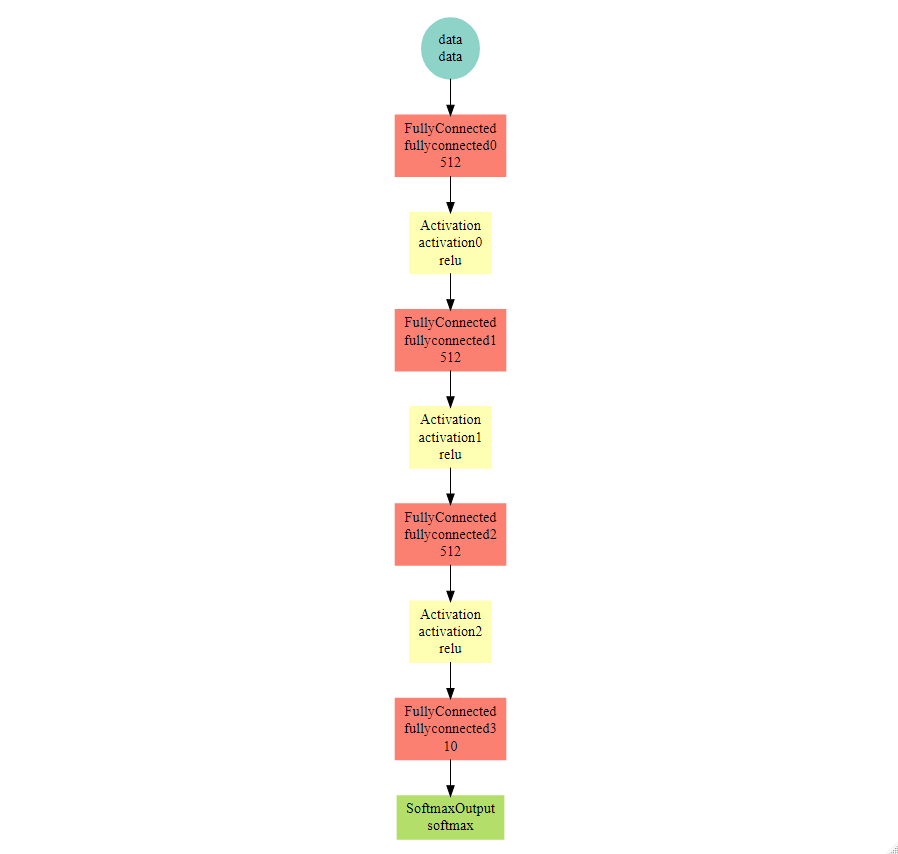
\includegraphics[width= 8.7cm, height=7.7cm]{figure/mxnet_graph_decay.png}
\end{figure}
\end{minipage}
\framebreak
%%%%%%%%%%%%%%%%%%%%%%%%%%%%%%%%%%%%%%%%%%%%%%%%%%%%%%%%%%%%%%%%%%

\begin{figure}
\centering
\scalebox{1}{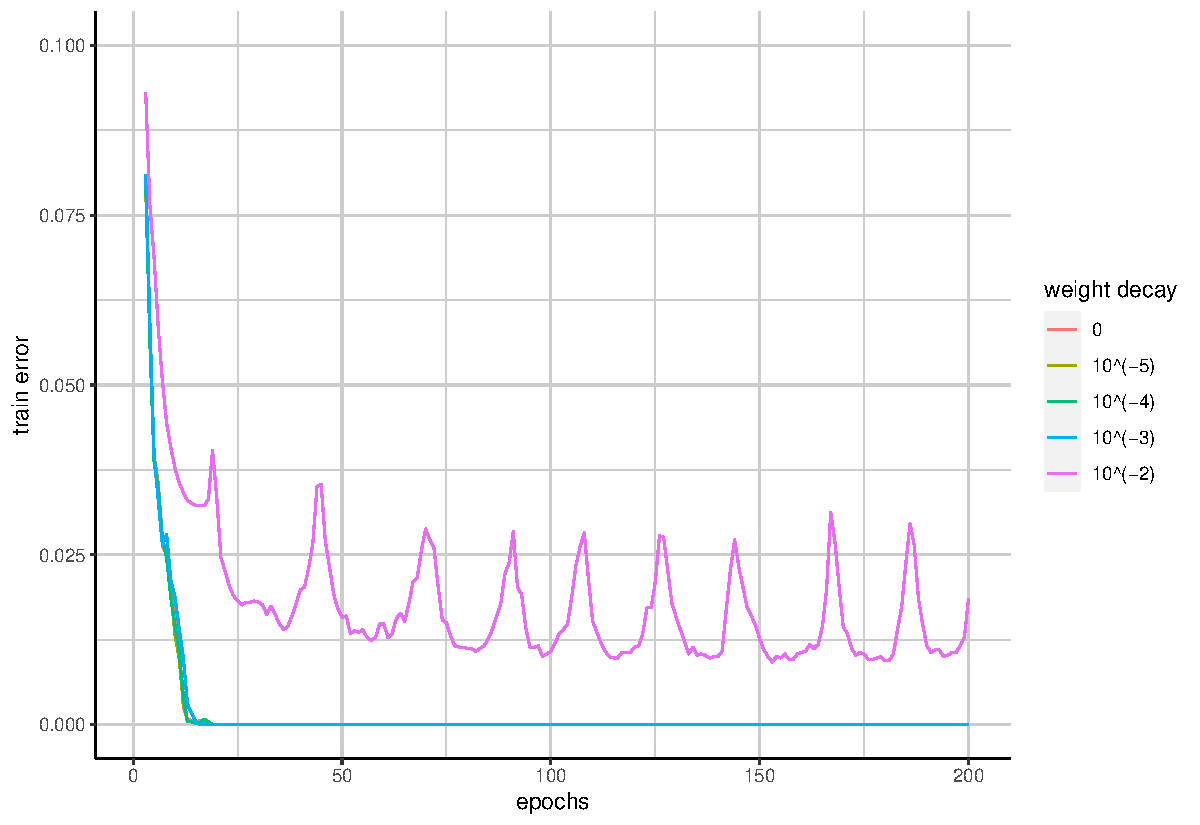
\includegraphics{figure_man/weight_decay1.pdf}}
\\
A high weight decay of $10^{-2}$ leads to a high error on the training data.
\end{figure}

\framebreak
%%%%%%%%%%%%%%%%%%%%%%%%%%%%%%%%%%%%%%%%%%%%%%%%%%%%%%%%%%%%%%%%%%

\begin{figure}
\centering
\scalebox{1}{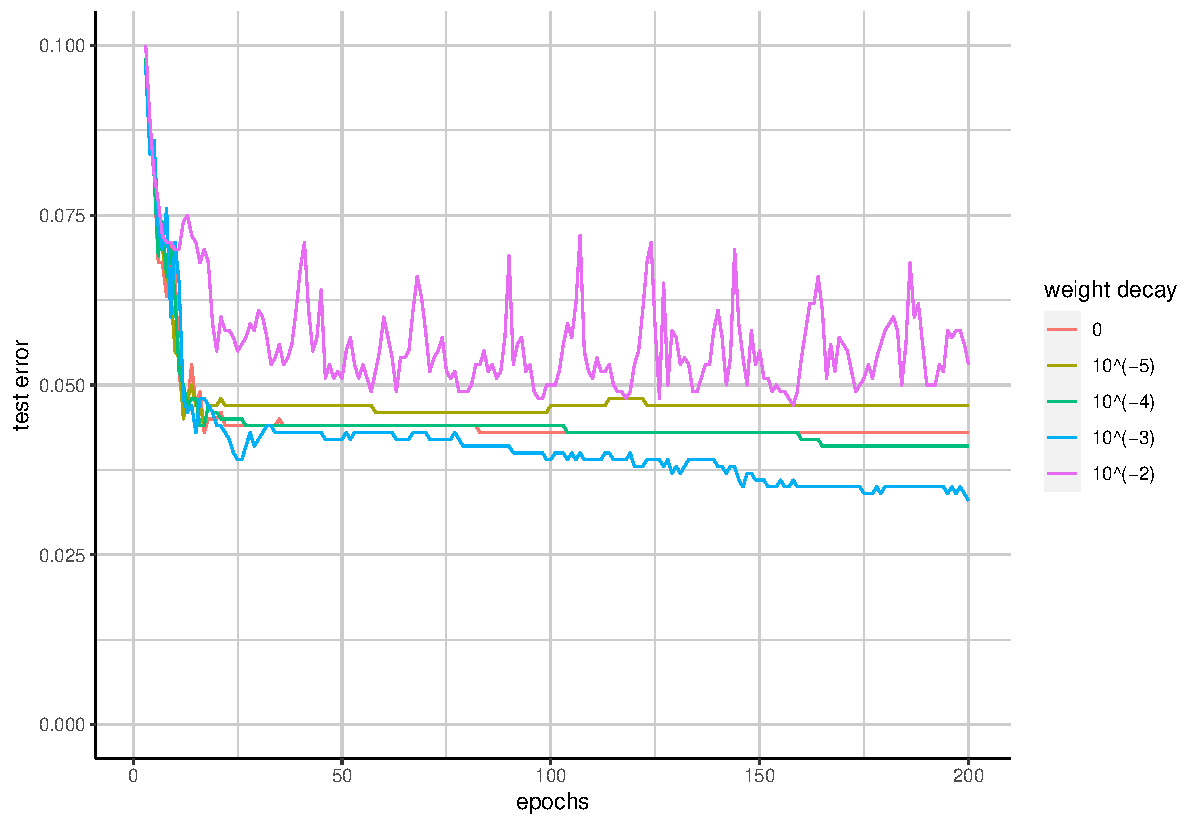
\includegraphics{figure_man/weight_decay2.pdf}}
\\
Second strongest weight decay leads to the best result on the test data.
\end{figure}
\end{vbframe}
  
%%%%%%%%%%%%%%%%%%%%%%%%%%%%%%%%%%%%%%%%%%%%%%%%%%%%%%%%%%%%%%%%%%
\begin{frame}{Tensorflow Playground}
\begin{figure}
\centering
\scalebox{0.8}{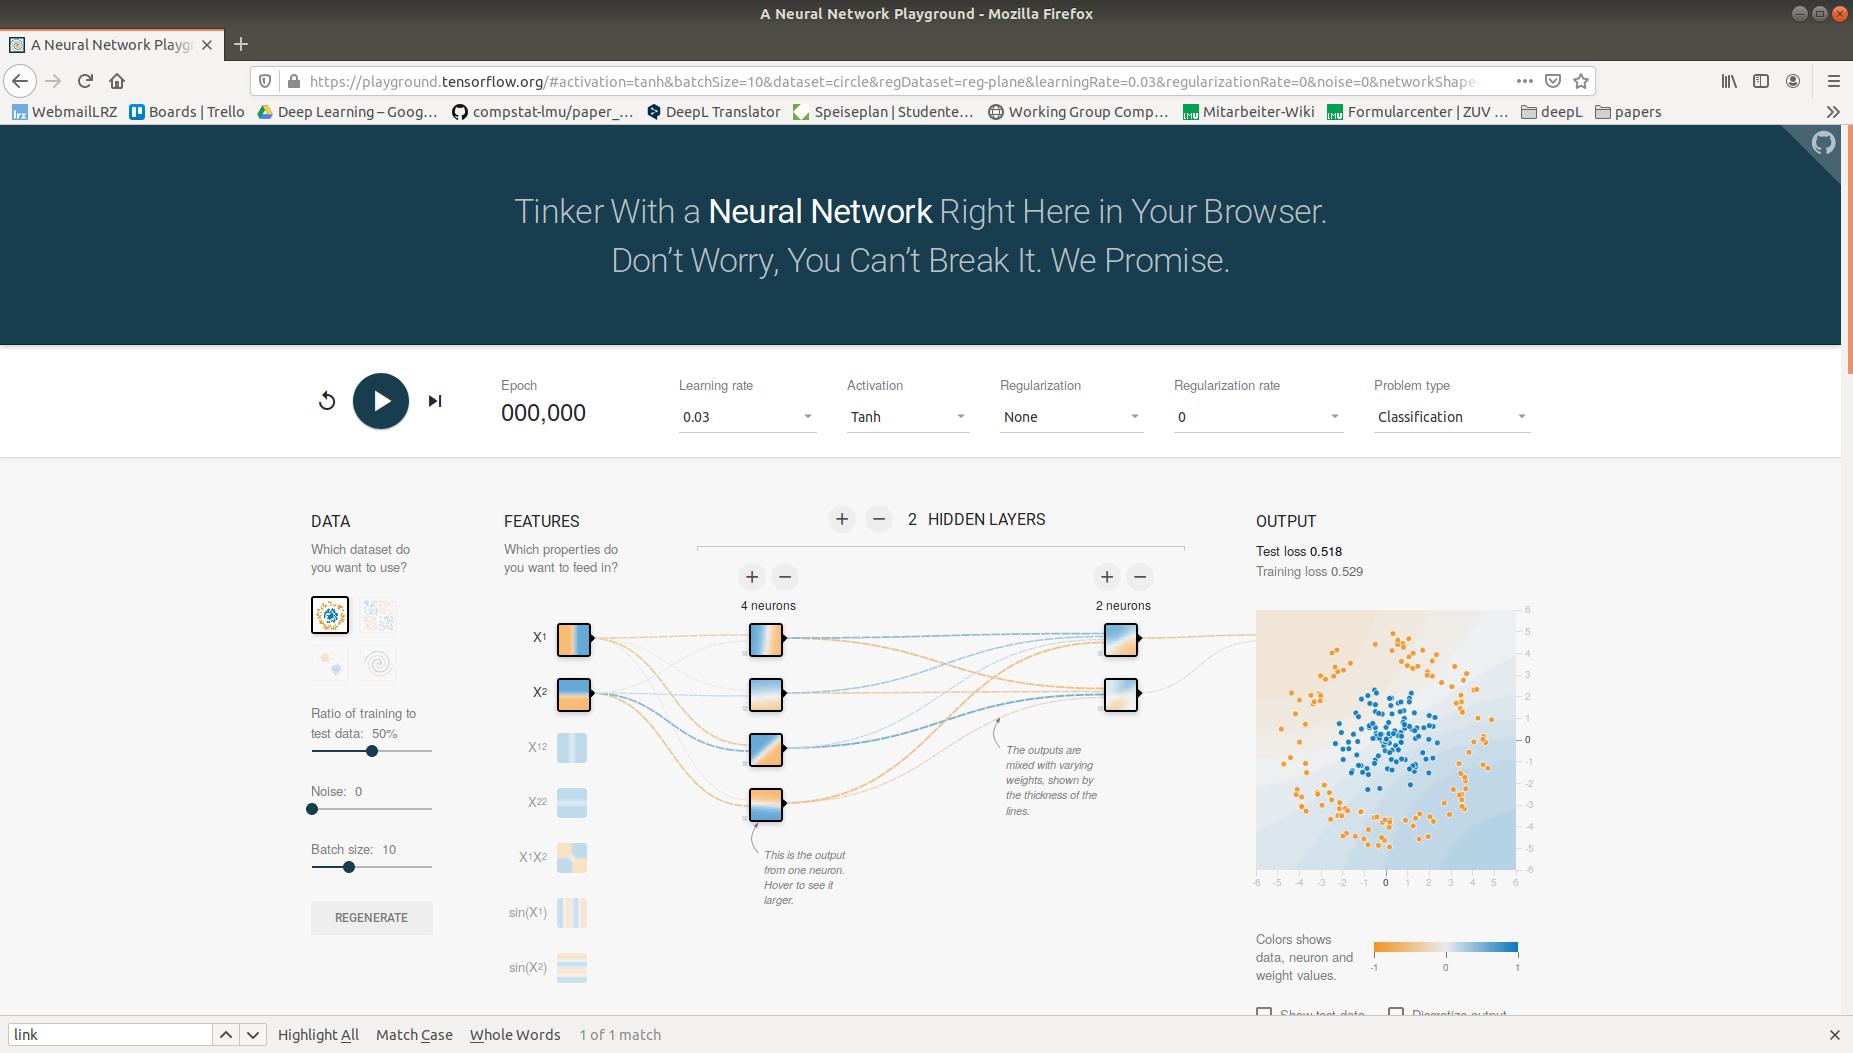
\includegraphics{figure/tensorflow_playground.png}}
  \caption{\url{https://playground.tensorflow.org/}, (Carter)}
  \end{figure}
\end{frame}

\begin{frame}{Tensorflow Playground - Exercise}
  \begin{figure}
    \centering
      \scalebox{0.8}{
\includegraphics{figure/tensorflow_exercise.png}}
    \caption{\url{https://developers.google.com/machine-learning/crash-course/regularization-for-simplicity/playground-exercise-examining-l2-regularization} (Google)}
  \end{figure}
\end{frame}

%%%%%%%%%%%%%%%%%%%%%%%%%%%%%%%%%%%%%%%%%%%%%%%%%%%%%%%%%%%%%%%%%%
%%%%%%%%%%%%%%%%%%%%%%%%%%%%%%%%%%%%%%%%%%%%%%%%%%%%%%%%%%%%%%%%%%
%%%%%%%%%%%%%%%%%%          REFERENCES          %%%%%%%%%%%%%%%%%%
%%%%%%%%%%%%%%%%%%%%%%%%%%%%%%%%%%%%%%%%%%%%%%%%%%%%%%%%%%%%%%%%%%
\begin{vbframe}
\frametitle{References}
\footnotesize{
\begin{thebibliography}{99}
%%%%%%%%%%%%%%%%%%%%%%%%%%%%%%%%%%
\bibitem[(Goodfellow, 2016)]{1} 
Goodfellow, I., Bengio, Y., \& Courville, A. (2016). \textit{Deep Learning}. MIT Press. 
%%%%%%%%%%%%%%%%%%%%%%%%%%%%%%%%%%
\bibitem[(MathWorks)]{2} 
MathWorks. (n.d.). \textit{Regularization}. MATLAB \& Simulink. \url{https://de.mathworks.com/discovery/regularization.html}
%%%%%%%%%%%%%%%%%%%%%%%%%%%%%%%%%%
\bibitem[(Carter)]{3} 
Carter, D. S. and S. (n.d.). \textit{Tensorflow - Neural Network Playground. A Neural Network Playground}. \url{https://playground.tensorflow.org} 
%%%%%%%%%%%%%%%%%%%%%%%%%%%%%%%%%%
\bibitem[(Google)]{4} Google. (n.d.). \textit{Regularization for Simplicity: Playground Exercise (L2 Regularization)}. Google. \url{https://developers.google.com/machine-learning/crash-course/regularization-for-simplicity/playground-exercise-examining-l2-regularization?hl=de} 
\end{thebibliography}
}
\end{vbframe}
%%%%%%%%%%%%%%%%%%%%%%%%%%%%%%%%%%%%%%%%%%%%%%%%%%%%%%%%%%%%%%%%%%
%%%%%%%%%%%%%%%%%%%%%%%%%%%%%%%%%%%%%%%%%%%%%%%%%%%%%%%%%%%%%%%%%%

\endlecture
\end{document}